\chapter{Aportaciones}

\section{Redes Neuronales Totalmente Conectadas}
\subsection{BackPropagation con 1 capa oculta}

\begin{figure}[H]
	\centering
	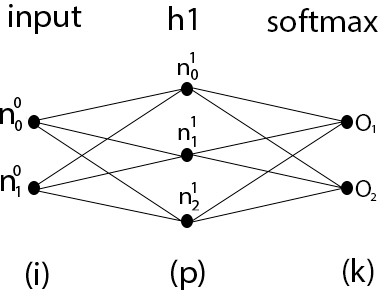
\includegraphics[scale=0.35]{imagenes/nn_1_capa.jpg}  
	\caption{Red Neuronal totalmente conectada con 1 capa oculta}
	\label{fig:nn_1_capa}
\end{figure}

La Figura 2.1 se compone de puntos y líneas, representando neuronas y pesos que las conectan respectivamente. Cada punto es una neurona, y cada línea un peso. \\
El peso $W_{ip}$ referencia al peso que une las neuronas $X_i$ y $h_p$.\\
El peso $W_{p\hat{y}}$ representa el peso que conecta las neuronas $h_p$ y $\hat{y}$.


\subsubsection{Capa output}

Sea la neurona $n$, se define como $n_{in}$ el valor de dicha neurona antes de aplicar sobre ella su función de activación asociada, y $n_{out}$ el obtenido tras aplicarla.
De esta forma, si la última capa es $\hat{y}$ y solo tiene una neurona, $\hat{y_{in}}$ y $\hat{y_{out}}$ corresponderán con los valores antes y después de aplicar la función de activación respectivamente.\\

De esta forma, la función de pérdida (2.1) se convierte en:

\begin{gather}
	H(x) = - \frac{1}{N} \sum_{i=1}^{N}  [y_i * log( \hat{y}_{out_i}) + (1-y_i)*log(1-\hat{y}_{out_i})]
\end{gather}

Para realizar el descenso del gradiente, se debe empezar calculando la derivada de la función de pérdida respecto a la predicción obtenida. Es decir, la derivada de la fórmula (2.2) respecto de las neuronas en la última capa de la red tras aplicar sus respectivas funciones de activación, que en este caso corresponde a $\hat{y}_{out}$. \\
Por simplicidad, podemos dividir esta derivada en 2 partes. \\
Parte izquierda:
\begin{gather}
	f(x) = A*B \\  
	f'(x) = AB' + A'B \\
	\frac{dy_i}{d\hat{y}_{out_i}} = 0 \\
	\frac{dlog(\hat{y}_{out_i} )}{d\hat{y}_{out_i}} = \frac{1}{\hat{y}_{out_i}} \\
	\frac{dy_i * log( \hat{y}_{out_i})}{d\hat{y}_{out_i}} = y_i*\frac{1}{\hat{y}_{out_i}} + 0*log(\hat{y}_{out_i} ) = \frac{y_i}{\hat{y}_{out_i}}
\end{gather}

Parte derecha:
\begin{gather}
	\frac{d(1-y_i)}{d\hat{y}_{out_i}} = 0\\
	\frac{dlog(1-\hat{y}_{out_i})}{d\hat{y}_{out_i}} = \frac{1}{1-\hat{y}_{out_i}} * (-1) \\
	\frac{d(1-y_i)*log(1-\hat{y}_{out_i})}{d\hat{y}_{out_i}} = (1-y_i)*\frac{1}{1-\hat{y}_{out_i}}*(-1) + 0* log(1-\hat{y}_{out_i}) \\
	\frac{d(1-y_i)*log(1-\hat{y}_{out_i})}{d\hat{y}_{out_i}} = -\frac{1-y_i}{1-\hat{y}_{out_i}}
\end{gather}

Finalmente, se obtiene: 
\begin{gather}
	\frac{dH(x)}{d\hat{y}_{out_i}} = - \frac{1}{N} \sum_{i=1}^{N}  [ \frac{y_i}{\hat{y}_{out_i}} - \frac{1-y_i}{1-\hat{y}_{out_i}} ]
\end{gather}

\subsubsection{Función activación de la capa output}
En la capa output se emplea la función de activación sigmoide. 

\begin{gather}
	sigmoide(x) = \frac{1}{1+e^{-x}} \\
	sigmoide'(x) = \frac{sigmoide(x)}{1-sigmoide(x)}
\end{gather}

De esta forma,

\begin{gather}
	\frac{d\hat{y}_{out}}{d\hat{y}_{in}} = \frac{d sigmoide(\hat{y}_{in})}{d\hat{y}_{in}} = sigmoide(\hat{y}_{in})*(1-sigmoide(\hat{y}_{in}))
\end{gather}

Ahora, podemos calcular el gradiente completo hasta la capa output antes de aplicar su función de activación.

\begin{gather}
	grad\_output = \frac{dH(x)}{d\hat{y}_{out}} * \frac{d\hat{y}_{out}}{d\hat{y}_{in}} =
	- \frac{1}{N} \sum_{i=1}^{N}  [ \frac{y_i}{\hat{y}_{out_i}} - \frac{1-y_i}{1-\hat{y}_{out_i}} ] * \frac{d\hat{y}_{out}}{d\hat{y}_{in}} \\
	grad\_output = - \frac{1}{N} \sum_{i=1}^{N}  [ \frac{y_i}{\hat{y}_{out_i}} - \frac{1-y_i}{1-\hat{y}_{out_i}} ] * sigmoide(\hat{y}_{in})*(1-sigmoide(\hat{y}_{in}))
\end{gather}

\subsubsection{Pesos capas h1-output}

Una vez calculado el gradiente hasta la capa output, se puede calcular el gradiente respecto a cada peso que se encuentra conectado a esta desde la capa anterior. Es decir, para cada $h_p\in h1$, se calcula $\frac{dH(x)}{dW_{p\hat{y}}}$. Usando la regla de la cadena, equivale a realizar lo siguiente:

\begin{gather}
	\frac{d\hat{y}_{in}}{dW_{p\hat{y}}} = \frac{dh_{1out_p} * W_{p\hat{y}}}{dW_{p\hat{y}}} = h_{1out_p} \\
	\frac{dH(x)}{dW_{p\hat{y}}} = \frac{dH(x)}{d\hat{y}_{out}} * \frac{d\hat{y}_{out}}{d\hat{y}_{in}} * \frac{d\hat{y}_{in}}{dW_{p\hat{y}}} =  grad\_output * \frac{d\hat{y}_{in}}{dW_{p\hat{y}}} = grad\_output * h_{1out_p}
\end{gather}

\subsubsection{Capa oculta h1}

\subsubsection{Capa input}